Insert your text here. This is an AI-generated text as an example of how your text will look like in the document.

The convergence of biology and technology marks a new era in scientific exploration. Biotechnology, in particular, has become a pivotal field, harnessing cellular and biomolecular processes to develop technologies and products that help improve our lives and the health of our planet. Genetic engineering, for example, has enabled the creation of crops that are more resistant to pests and diseases, reducing the need for chemical pesticides and enhancing food security for a growing global population.

Simultaneously, the realm of computer science has evolved dramatically, giving rise to artificial intelligence (AI) and machine learning. These technologies are not just transforming the way we live and work but are also revolutionizing scientific research. AI algorithms can process and analyze data at speeds and scales unimaginable to the human brain, uncovering patterns and insights that accelerate innovation in fields ranging from medicine to environmental science. The integration of AI in research methodologies is enabling faster, more accurate predictions and solutions to complex problems.

Furthermore, the importance of sustainability in scientific research has come to the forefront. Scientists are increasingly focused on developing technologies and processes that are environmentally friendly and sustainable over the long term. Renewable energy sources such as solar and wind power are being refined to replace fossil fuels, while advancements in materials science are leading to the creation of biodegradable plastics and more efficient batteries. This shift towards sustainability not only addresses the urgent challenge of climate change but also paves the way for a healthier, more sustainable future for all.

As we look forward, the intersection of different scientific disciplines promises to usher in a new age of discovery and innovation. The collaboration between fields such as genetics, nanotechnology, and environmental science is breaking down traditional barriers and fostering a holistic approach to solving the world's most pressing issues. In this ever-evolving landscape, the potential for scientific breakthroughs is limitless, reminding us of the power of human curiosity and the endless possibilities that lie ahead.

\section{Introduction}
\subsection{Subsection title}


This is an example figure:

 \begin{figure}[h!]
	\centering
	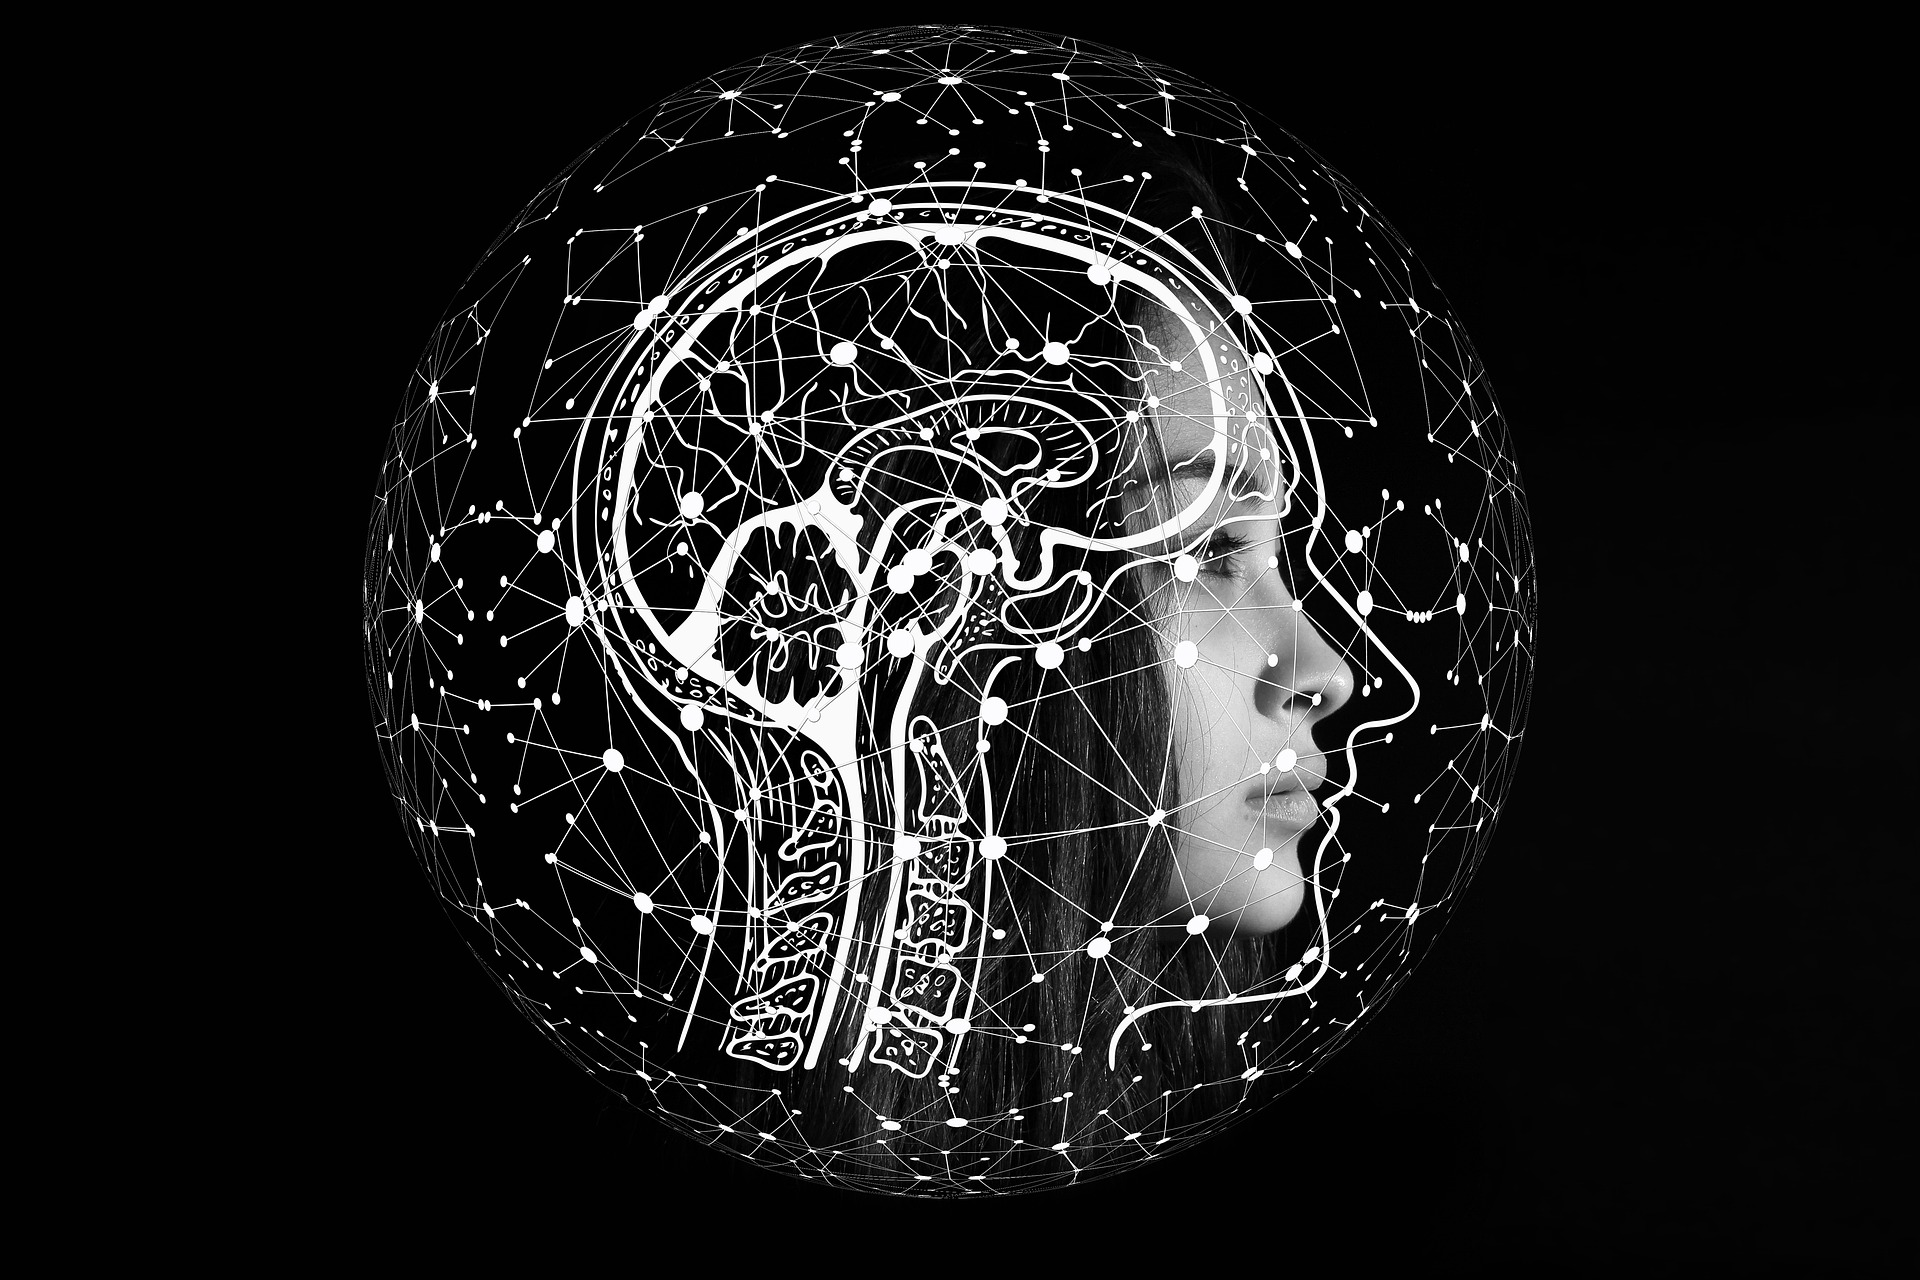
\includegraphics{examplefigure}
	\caption{This is an example figure.}
	\label{figurelabel}	 
\end{figure}

This is an example equation:

\begin{equation}
	\sigma = \frac{1}{kT} \sum_i n_i q_i^2 D_i
\end{equation}

You can refer to a figure in the middle of the text by typing \ref{figurelabel}

You can connect your bibliography to zotero and cite your references in the text with cite function \cite{referencename}. 

\section{Aim of the work}

 Insert your text here.

\section{Title of results section}
 \subsection{Title of subsection}
 
 Insert your text here.
 
 \section{Title of results section}
 \subsection{Title of subsection}

 Insert your text here.


\clearpage
\section{Conclusions and perspectives}

Insert your conclusions here. 

%%%%%%References%%%%%%
\printbibliography[heading=bibliography, title={References}]


